% Options for packages loaded elsewhere
% Options for packages loaded elsewhere
\PassOptionsToPackage{unicode}{hyperref}
\PassOptionsToPackage{hyphens}{url}
\PassOptionsToPackage{dvipsnames,svgnames,x11names}{xcolor}
%
\documentclass[
  letterpaper,
  DIV=11,
  numbers=noendperiod]{scrartcl}
\usepackage{xcolor}
\usepackage{amsmath,amssymb}
\setcounter{secnumdepth}{-\maxdimen} % remove section numbering
\usepackage{iftex}
\ifPDFTeX
  \usepackage[T1]{fontenc}
  \usepackage[utf8]{inputenc}
  \usepackage{textcomp} % provide euro and other symbols
\else % if luatex or xetex
  \usepackage{unicode-math} % this also loads fontspec
  \defaultfontfeatures{Scale=MatchLowercase}
  \defaultfontfeatures[\rmfamily]{Ligatures=TeX,Scale=1}
\fi
\usepackage{lmodern}
\ifPDFTeX\else
  % xetex/luatex font selection
\fi
% Use upquote if available, for straight quotes in verbatim environments
\IfFileExists{upquote.sty}{\usepackage{upquote}}{}
\IfFileExists{microtype.sty}{% use microtype if available
  \usepackage[]{microtype}
  \UseMicrotypeSet[protrusion]{basicmath} % disable protrusion for tt fonts
}{}
\makeatletter
\@ifundefined{KOMAClassName}{% if non-KOMA class
  \IfFileExists{parskip.sty}{%
    \usepackage{parskip}
  }{% else
    \setlength{\parindent}{0pt}
    \setlength{\parskip}{6pt plus 2pt minus 1pt}}
}{% if KOMA class
  \KOMAoptions{parskip=half}}
\makeatother
% Make \paragraph and \subparagraph free-standing
\makeatletter
\ifx\paragraph\undefined\else
  \let\oldparagraph\paragraph
  \renewcommand{\paragraph}{
    \@ifstar
      \xxxParagraphStar
      \xxxParagraphNoStar
  }
  \newcommand{\xxxParagraphStar}[1]{\oldparagraph*{#1}\mbox{}}
  \newcommand{\xxxParagraphNoStar}[1]{\oldparagraph{#1}\mbox{}}
\fi
\ifx\subparagraph\undefined\else
  \let\oldsubparagraph\subparagraph
  \renewcommand{\subparagraph}{
    \@ifstar
      \xxxSubParagraphStar
      \xxxSubParagraphNoStar
  }
  \newcommand{\xxxSubParagraphStar}[1]{\oldsubparagraph*{#1}\mbox{}}
  \newcommand{\xxxSubParagraphNoStar}[1]{\oldsubparagraph{#1}\mbox{}}
\fi
\makeatother

\usepackage{color}
\usepackage{fancyvrb}
\newcommand{\VerbBar}{|}
\newcommand{\VERB}{\Verb[commandchars=\\\{\}]}
\DefineVerbatimEnvironment{Highlighting}{Verbatim}{commandchars=\\\{\}}
% Add ',fontsize=\small' for more characters per line
\usepackage{framed}
\definecolor{shadecolor}{RGB}{241,243,245}
\newenvironment{Shaded}{\begin{snugshade}}{\end{snugshade}}
\newcommand{\AlertTok}[1]{\textcolor[rgb]{0.68,0.00,0.00}{#1}}
\newcommand{\AnnotationTok}[1]{\textcolor[rgb]{0.37,0.37,0.37}{#1}}
\newcommand{\AttributeTok}[1]{\textcolor[rgb]{0.40,0.45,0.13}{#1}}
\newcommand{\BaseNTok}[1]{\textcolor[rgb]{0.68,0.00,0.00}{#1}}
\newcommand{\BuiltInTok}[1]{\textcolor[rgb]{0.00,0.23,0.31}{#1}}
\newcommand{\CharTok}[1]{\textcolor[rgb]{0.13,0.47,0.30}{#1}}
\newcommand{\CommentTok}[1]{\textcolor[rgb]{0.37,0.37,0.37}{#1}}
\newcommand{\CommentVarTok}[1]{\textcolor[rgb]{0.37,0.37,0.37}{\textit{#1}}}
\newcommand{\ConstantTok}[1]{\textcolor[rgb]{0.56,0.35,0.01}{#1}}
\newcommand{\ControlFlowTok}[1]{\textcolor[rgb]{0.00,0.23,0.31}{\textbf{#1}}}
\newcommand{\DataTypeTok}[1]{\textcolor[rgb]{0.68,0.00,0.00}{#1}}
\newcommand{\DecValTok}[1]{\textcolor[rgb]{0.68,0.00,0.00}{#1}}
\newcommand{\DocumentationTok}[1]{\textcolor[rgb]{0.37,0.37,0.37}{\textit{#1}}}
\newcommand{\ErrorTok}[1]{\textcolor[rgb]{0.68,0.00,0.00}{#1}}
\newcommand{\ExtensionTok}[1]{\textcolor[rgb]{0.00,0.23,0.31}{#1}}
\newcommand{\FloatTok}[1]{\textcolor[rgb]{0.68,0.00,0.00}{#1}}
\newcommand{\FunctionTok}[1]{\textcolor[rgb]{0.28,0.35,0.67}{#1}}
\newcommand{\ImportTok}[1]{\textcolor[rgb]{0.00,0.46,0.62}{#1}}
\newcommand{\InformationTok}[1]{\textcolor[rgb]{0.37,0.37,0.37}{#1}}
\newcommand{\KeywordTok}[1]{\textcolor[rgb]{0.00,0.23,0.31}{\textbf{#1}}}
\newcommand{\NormalTok}[1]{\textcolor[rgb]{0.00,0.23,0.31}{#1}}
\newcommand{\OperatorTok}[1]{\textcolor[rgb]{0.37,0.37,0.37}{#1}}
\newcommand{\OtherTok}[1]{\textcolor[rgb]{0.00,0.23,0.31}{#1}}
\newcommand{\PreprocessorTok}[1]{\textcolor[rgb]{0.68,0.00,0.00}{#1}}
\newcommand{\RegionMarkerTok}[1]{\textcolor[rgb]{0.00,0.23,0.31}{#1}}
\newcommand{\SpecialCharTok}[1]{\textcolor[rgb]{0.37,0.37,0.37}{#1}}
\newcommand{\SpecialStringTok}[1]{\textcolor[rgb]{0.13,0.47,0.30}{#1}}
\newcommand{\StringTok}[1]{\textcolor[rgb]{0.13,0.47,0.30}{#1}}
\newcommand{\VariableTok}[1]{\textcolor[rgb]{0.07,0.07,0.07}{#1}}
\newcommand{\VerbatimStringTok}[1]{\textcolor[rgb]{0.13,0.47,0.30}{#1}}
\newcommand{\WarningTok}[1]{\textcolor[rgb]{0.37,0.37,0.37}{\textit{#1}}}

\usepackage{longtable,booktabs,array}
\usepackage{calc} % for calculating minipage widths
% Correct order of tables after \paragraph or \subparagraph
\usepackage{etoolbox}
\makeatletter
\patchcmd\longtable{\par}{\if@noskipsec\mbox{}\fi\par}{}{}
\makeatother
% Allow footnotes in longtable head/foot
\IfFileExists{footnotehyper.sty}{\usepackage{footnotehyper}}{\usepackage{footnote}}
\makesavenoteenv{longtable}
\usepackage{graphicx}
\makeatletter
\newsavebox\pandoc@box
\newcommand*\pandocbounded[1]{% scales image to fit in text height/width
  \sbox\pandoc@box{#1}%
  \Gscale@div\@tempa{\textheight}{\dimexpr\ht\pandoc@box+\dp\pandoc@box\relax}%
  \Gscale@div\@tempb{\linewidth}{\wd\pandoc@box}%
  \ifdim\@tempb\p@<\@tempa\p@\let\@tempa\@tempb\fi% select the smaller of both
  \ifdim\@tempa\p@<\p@\scalebox{\@tempa}{\usebox\pandoc@box}%
  \else\usebox{\pandoc@box}%
  \fi%
}
% Set default figure placement to htbp
\def\fps@figure{htbp}
\makeatother





\setlength{\emergencystretch}{3em} % prevent overfull lines

\providecommand{\tightlist}{%
  \setlength{\itemsep}{0pt}\setlength{\parskip}{0pt}}



 


\usepackage{booktabs}
\usepackage{longtable}
\usepackage{array}
\usepackage{multirow}
\usepackage{wrapfig}
\usepackage{float}
\usepackage{colortbl}
\usepackage{pdflscape}
\usepackage{tabu}
\usepackage{threeparttable}
\usepackage{threeparttablex}
\usepackage[normalem]{ulem}
\usepackage{makecell}
\usepackage{xcolor}
\KOMAoption{captions}{tableheading}
\makeatletter
\@ifpackageloaded{caption}{}{\usepackage{caption}}
\AtBeginDocument{%
\ifdefined\contentsname
  \renewcommand*\contentsname{Table of contents}
\else
  \newcommand\contentsname{Table of contents}
\fi
\ifdefined\listfigurename
  \renewcommand*\listfigurename{List of Figures}
\else
  \newcommand\listfigurename{List of Figures}
\fi
\ifdefined\listtablename
  \renewcommand*\listtablename{List of Tables}
\else
  \newcommand\listtablename{List of Tables}
\fi
\ifdefined\figurename
  \renewcommand*\figurename{Figure}
\else
  \newcommand\figurename{Figure}
\fi
\ifdefined\tablename
  \renewcommand*\tablename{Table}
\else
  \newcommand\tablename{Table}
\fi
}
\@ifpackageloaded{float}{}{\usepackage{float}}
\floatstyle{ruled}
\@ifundefined{c@chapter}{\newfloat{codelisting}{h}{lop}}{\newfloat{codelisting}{h}{lop}[chapter]}
\floatname{codelisting}{Listing}
\newcommand*\listoflistings{\listof{codelisting}{List of Listings}}
\makeatother
\makeatletter
\makeatother
\makeatletter
\@ifpackageloaded{caption}{}{\usepackage{caption}}
\@ifpackageloaded{subcaption}{}{\usepackage{subcaption}}
\makeatother
\usepackage{bookmark}
\IfFileExists{xurl.sty}{\usepackage{xurl}}{} % add URL line breaks if available
\urlstyle{same}
\hypersetup{
  pdftitle={Effect of a WNBA Team on Girls' Sports Participation},
  pdfauthor={Tate Mason},
  colorlinks=true,
  linkcolor={blue},
  filecolor={Maroon},
  citecolor={Blue},
  urlcolor={Blue},
  pdfcreator={LaTeX via pandoc}}


\title{Effect of a WNBA Team on Girls' Sports Participation}
\author{Tate Mason}
\date{Invalid Date}
\begin{document}
\maketitle


\section{Introduction}\label{introduction}

This file serves as the data analysis portion of my project. I will be
using NFHS data and WNBA data sourced from Kaggle to analyze the effect
of a WNBA team on the youth sports participation of girls in a given
state. I will be focusing on Basketball, Track, and Softball, as these
are the most available sports in\\
WFHS.

\section{Data Cleaning}\label{data-cleaning}

NFHS data was cleaned by Claude Code, scraping PDF's and converting to
CSV's. WNBA data is downloaded clean. Still, I want to make sure things
are formatted correctly.

\begin{Shaded}
\begin{Highlighting}[]
\FunctionTok{library}\NormalTok{(tidyverse)}
\end{Highlighting}
\end{Shaded}

\begin{verbatim}
-- Attaching core tidyverse packages ------------------------ tidyverse 2.0.0 --
v dplyr     1.1.4     v readr     2.1.5
v forcats   1.0.0     v stringr   1.5.2
v ggplot2   4.0.0     v tibble    3.3.0
v lubridate 1.9.4     v tidyr     1.3.1
v purrr     1.1.0     
-- Conflicts ------------------------------------------ tidyverse_conflicts() --
x dplyr::filter() masks stats::filter()
x dplyr::lag()    masks stats::lag()
i Use the conflicted package (<http://conflicted.r-lib.org/>) to force all conflicts to become errors
\end{verbatim}

\begin{Shaded}
\begin{Highlighting}[]
\FunctionTok{library}\NormalTok{(readr)}
\FunctionTok{library}\NormalTok{(ggplot2)}
\FunctionTok{library}\NormalTok{(knitr)}
\FunctionTok{library}\NormalTok{(kableExtra)}
\end{Highlighting}
\end{Shaded}

\begin{verbatim}

Attaching package: 'kableExtra'

The following object is masked from 'package:dplyr':

    group_rows
\end{verbatim}

\begin{Shaded}
\begin{Highlighting}[]
\FunctionTok{library}\NormalTok{(psych)}
\end{Highlighting}
\end{Shaded}

\begin{verbatim}

Attaching package: 'psych'

The following objects are masked from 'package:ggplot2':

    %+%, alpha
\end{verbatim}

\begin{Shaded}
\begin{Highlighting}[]
\NormalTok{df\_wnba }\OtherTok{\textless{}{-}} \FunctionTok{read\_csv}\NormalTok{(}\StringTok{"\textasciitilde{}/SchoolWork/Y2S2/Health/ResProj/Data/WNBA\_Standings.csv"}\NormalTok{)}
\end{Highlighting}
\end{Shaded}

\begin{verbatim}
Rows: 352 Columns: 13
-- Column specification --------------------------------------------------------
Delimiter: ","
chr (8): TEAM, CONF, DIV, HOME, ROAD, OT, LAST 10, STREAK
dbl (5): RANK, W, L, WIN%, YEAR

i Use `spec()` to retrieve the full column specification for this data.
i Specify the column types or set `show_col_types = FALSE` to quiet this message.
\end{verbatim}

\begin{Shaded}
\begin{Highlighting}[]
\NormalTok{df\_nfhs\_wide }\OtherTok{\textless{}{-}} \FunctionTok{read\_csv}\NormalTok{(}\StringTok{"\textasciitilde{}/SchoolWork/Y2S2/Health/ResProj/Data/NFHS/nfhs\_processed/state\_sport\_participation\_wide.csv"}\NormalTok{)}
\end{Highlighting}
\end{Shaded}

\begin{verbatim}
Rows: 1715 Columns: 26
-- Column specification --------------------------------------------------------
Delimiter: ","
chr  (3): survey_year, gender, state
dbl (23): Baseball, Basketball, Bowling, Competitive Spirit Squads, Cross Co...

i Use `spec()` to retrieve the full column specification for this data.
i Specify the column types or set `show_col_types = FALSE` to quiet this message.
\end{verbatim}

\begin{Shaded}
\begin{Highlighting}[]
\CommentTok{\# Looking at WNBA data}

\NormalTok{dummy }\OtherTok{\textless{}{-}} \FunctionTok{rep}\NormalTok{(}\FunctionTok{c}\NormalTok{(}\DecValTok{1}\NormalTok{,}\DecValTok{0}\NormalTok{), }\AttributeTok{length.out =} \FunctionTok{nrow}\NormalTok{(df\_wnba))}
\NormalTok{df\_wnba }\OtherTok{\textless{}{-}}\NormalTok{ df\_wnba }\SpecialCharTok{\%\textgreater{}\%}
  \FunctionTok{rename\_with}\NormalTok{(tolower) }\SpecialCharTok{\%\textgreater{}\%}
  \FunctionTok{mutate}\NormalTok{(}\AttributeTok{east =}\NormalTok{ dummy,}
         \AttributeTok{west =} \DecValTok{1} \SpecialCharTok{{-}}\NormalTok{ dummy) }\SpecialCharTok{\%\textgreater{}\%}
  \FunctionTok{filter}\NormalTok{(year }\SpecialCharTok{\textless{}=} \DecValTok{2019}\NormalTok{)}
\FunctionTok{head}\NormalTok{(df\_wnba)}
\end{Highlighting}
\end{Shaded}

\begin{verbatim}
# A tibble: 6 x 15
   rank team       w     l `win%` conf  div   home  road  ot    `last 10` streak
  <dbl> <chr>  <dbl> <dbl>  <dbl> <chr> <chr> <chr> <chr> <chr> <chr>     <chr> 
1     1 NEW Y~    17    11  0.607 5-3   0-0   10-4  7-7   0-0   3-7       W 1   
2     1 HOUST~    18    10  0.643 12-4  0-0   9-5   9-5   0-0   7-3       L 2   
3     2 CHARL~    15    13  0.536 4-4   0-0   12-2  3-11  0-0   5-5       W 1   
4     2 PHOEN~    16    12  0.571 10-6  0-0   11-3  5-9   0-0   7-3       W 3   
5     3 CLEVE~    15    13  0.536 3-5   0-0   8-6   7-7   0-0   5-5       L 1   
6     3 LOS A~    14    14  0.5   9-7   0-0   8-6   6-8   0-0   6-4       L 1   
# i 3 more variables: year <dbl>, east <dbl>, west <dbl>
\end{verbatim}

\begin{Shaded}
\begin{Highlighting}[]
\FunctionTok{summary}\NormalTok{(df\_wnba)}
\end{Highlighting}
\end{Shaded}

\begin{verbatim}
      rank            team                 w               l        
 Min.   : 1.000   Length:292         Min.   : 3.00   Min.   : 3.00  
 1st Qu.: 2.000   Class :character   1st Qu.:13.00   1st Qu.:13.00  
 Median : 4.000   Mode  :character   Median :17.00   Median :16.00  
 Mean   : 4.248                      Mean   :16.64   Mean   :16.64  
 3rd Qu.: 6.000                      3rd Qu.:20.00   3rd Qu.:20.00  
 Max.   :12.000                      Max.   :29.00   Max.   :31.00  
 NA's   :14                                                         
      win%            conf               div                home          
 Min.   :0.0880   Length:292         Length:292         Length:292        
 1st Qu.:0.4045   Class :character   Class :character   Class :character  
 Median :0.5000   Mode  :character   Mode  :character   Mode  :character  
 Mean   :0.5000                                                           
 3rd Qu.:0.6180                                                           
 Max.   :0.9000                                                           
                                                                          
     road                ot              last 10             streak         
 Length:292         Length:292         Length:292         Length:292        
 Class :character   Class :character   Class :character   Class :character  
 Mode  :character   Mode  :character   Mode  :character   Mode  :character  
                                                                            
                                                                            
                                                                            
                                                                            
      year           east          west    
 Min.   :1997   Min.   :0.0   Min.   :0.0  
 1st Qu.:2002   1st Qu.:0.0   1st Qu.:0.0  
 Median :2008   Median :0.5   Median :0.5  
 Mean   :2008   Mean   :0.5   Mean   :0.5  
 3rd Qu.:2013   3rd Qu.:1.0   3rd Qu.:1.0  
 Max.   :2019   Max.   :1.0   Max.   :1.0  
                                           
\end{verbatim}

\begin{Shaded}
\begin{Highlighting}[]
\CommentTok{\# Looking at NFHS data}

\NormalTok{df\_nfhs\_wide }\OtherTok{\textless{}{-}}\NormalTok{ df\_nfhs\_wide }\SpecialCharTok{\%\textgreater{}\%}
  \FunctionTok{mutate}\NormalTok{(}
    \AttributeTok{gender =} \FunctionTok{case\_when}\NormalTok{(}
\NormalTok{      gender }\SpecialCharTok{==} \StringTok{"Boys"} \SpecialCharTok{\textasciitilde{}} \DecValTok{0}\NormalTok{,}
\NormalTok{      gender }\SpecialCharTok{==} \StringTok{"Girls"} \SpecialCharTok{\textasciitilde{}} \DecValTok{1}\NormalTok{,}
      \ConstantTok{TRUE} \SpecialCharTok{\textasciitilde{}} \ConstantTok{NA\_real\_}
\NormalTok{    ),}
    \AttributeTok{state =} \FunctionTok{case\_when}\NormalTok{(}
\NormalTok{      state }\SpecialCharTok{==} \StringTok{"Alabama"} \SpecialCharTok{\textasciitilde{}} \DecValTok{1}\NormalTok{,}
\NormalTok{      state }\SpecialCharTok{==} \StringTok{"Alaska"} \SpecialCharTok{\textasciitilde{}} \DecValTok{2}\NormalTok{,}
\NormalTok{      state }\SpecialCharTok{==} \StringTok{"Arizona"} \SpecialCharTok{\textasciitilde{}} \DecValTok{3}\NormalTok{,}
\NormalTok{      state }\SpecialCharTok{==} \StringTok{"Arkansas"} \SpecialCharTok{\textasciitilde{}} \DecValTok{4}\NormalTok{,}
\NormalTok{      state }\SpecialCharTok{==} \StringTok{"California"} \SpecialCharTok{\textasciitilde{}} \DecValTok{5}\NormalTok{,}
\NormalTok{      state }\SpecialCharTok{==} \StringTok{"Colorado"} \SpecialCharTok{\textasciitilde{}} \DecValTok{6}\NormalTok{,}
\NormalTok{      state }\SpecialCharTok{==} \StringTok{"Connecticut"} \SpecialCharTok{\textasciitilde{}} \DecValTok{7}\NormalTok{,}
\NormalTok{      state }\SpecialCharTok{==} \StringTok{"Delaware"} \SpecialCharTok{\textasciitilde{}} \DecValTok{8}\NormalTok{,}
\NormalTok{      state }\SpecialCharTok{==} \StringTok{"Florida"} \SpecialCharTok{\textasciitilde{}} \DecValTok{9}\NormalTok{,}
\NormalTok{      state }\SpecialCharTok{==} \StringTok{"Georgia"} \SpecialCharTok{\textasciitilde{}} \DecValTok{10}\NormalTok{,}
\NormalTok{      state }\SpecialCharTok{==} \StringTok{"Hawaii"} \SpecialCharTok{\textasciitilde{}} \DecValTok{11}\NormalTok{,}
\NormalTok{      state }\SpecialCharTok{==} \StringTok{"Idaho"} \SpecialCharTok{\textasciitilde{}} \DecValTok{12}\NormalTok{,}
\NormalTok{      state }\SpecialCharTok{==} \StringTok{"Illinois"} \SpecialCharTok{\textasciitilde{}} \DecValTok{13}\NormalTok{,}
\NormalTok{      state }\SpecialCharTok{==} \StringTok{"Indiana"} \SpecialCharTok{\textasciitilde{}} \DecValTok{14}\NormalTok{,}
\NormalTok{      state }\SpecialCharTok{==} \StringTok{"Iowa"} \SpecialCharTok{\textasciitilde{}} \DecValTok{15}\NormalTok{,}
\NormalTok{      state }\SpecialCharTok{==} \StringTok{"Kansas"} \SpecialCharTok{\textasciitilde{}} \DecValTok{16}\NormalTok{,}
\NormalTok{      state }\SpecialCharTok{==} \StringTok{"Kentucky"} \SpecialCharTok{\textasciitilde{}} \DecValTok{17}\NormalTok{,}
\NormalTok{      state }\SpecialCharTok{==} \StringTok{"Louisiana"} \SpecialCharTok{\textasciitilde{}} \DecValTok{18}\NormalTok{,}
\NormalTok{      state }\SpecialCharTok{==} \StringTok{"Maine"} \SpecialCharTok{\textasciitilde{}} \DecValTok{19}\NormalTok{,}
\NormalTok{      state }\SpecialCharTok{==} \StringTok{"Maryland"} \SpecialCharTok{\textasciitilde{}} \DecValTok{20}\NormalTok{,}
\NormalTok{      state }\SpecialCharTok{==} \StringTok{"Massachusetts"} \SpecialCharTok{\textasciitilde{}} \DecValTok{21}\NormalTok{,}
\NormalTok{      state }\SpecialCharTok{==} \StringTok{"Michigan"} \SpecialCharTok{\textasciitilde{}} \DecValTok{22}\NormalTok{,}
\NormalTok{      state }\SpecialCharTok{==} \StringTok{"Minnesota"} \SpecialCharTok{\textasciitilde{}} \DecValTok{23}\NormalTok{,}
\NormalTok{      state }\SpecialCharTok{==} \StringTok{"Mississippi"} \SpecialCharTok{\textasciitilde{}} \DecValTok{24}\NormalTok{,}
\NormalTok{      state }\SpecialCharTok{==} \StringTok{"Missouri"} \SpecialCharTok{\textasciitilde{}} \DecValTok{25}\NormalTok{,}
\NormalTok{      state }\SpecialCharTok{==} \StringTok{"Montana"} \SpecialCharTok{\textasciitilde{}} \DecValTok{26}\NormalTok{,}
\NormalTok{      state }\SpecialCharTok{==} \StringTok{"Nebraska"} \SpecialCharTok{\textasciitilde{}} \DecValTok{27}\NormalTok{,}
\NormalTok{      state }\SpecialCharTok{==} \StringTok{"Nevada"} \SpecialCharTok{\textasciitilde{}} \DecValTok{28}\NormalTok{,}
\NormalTok{      state }\SpecialCharTok{==} \StringTok{"New Hampshire"} \SpecialCharTok{\textasciitilde{}} \DecValTok{29}\NormalTok{,}
\NormalTok{      state }\SpecialCharTok{==} \StringTok{"New Jersey"} \SpecialCharTok{\textasciitilde{}} \DecValTok{30}\NormalTok{,}
\NormalTok{      state }\SpecialCharTok{==} \StringTok{"New Mexico"} \SpecialCharTok{\textasciitilde{}} \DecValTok{31}\NormalTok{,}
\NormalTok{      state }\SpecialCharTok{==} \StringTok{"New York"} \SpecialCharTok{\textasciitilde{}} \DecValTok{32}\NormalTok{,}
\NormalTok{      state }\SpecialCharTok{==} \StringTok{"North Carolina"} \SpecialCharTok{\textasciitilde{}} \DecValTok{33}\NormalTok{,}
\NormalTok{      state }\SpecialCharTok{==} \StringTok{"North Dakota"} \SpecialCharTok{\textasciitilde{}} \DecValTok{34}\NormalTok{,}
\NormalTok{      state }\SpecialCharTok{==} \StringTok{"Ohio"} \SpecialCharTok{\textasciitilde{}} \DecValTok{35}\NormalTok{,}
\NormalTok{      state }\SpecialCharTok{==} \StringTok{"Oklahoma"} \SpecialCharTok{\textasciitilde{}} \DecValTok{36}\NormalTok{,}
\NormalTok{      state }\SpecialCharTok{==} \StringTok{"Oregon"} \SpecialCharTok{\textasciitilde{}} \DecValTok{37}\NormalTok{,}
\NormalTok{      state }\SpecialCharTok{==} \StringTok{"Pennsylvania"} \SpecialCharTok{\textasciitilde{}} \DecValTok{38}\NormalTok{,}
\NormalTok{      state }\SpecialCharTok{==} \StringTok{"Rhode Island"} \SpecialCharTok{\textasciitilde{}} \DecValTok{39}\NormalTok{,}
\NormalTok{      state }\SpecialCharTok{==} \StringTok{"South Carolina"} \SpecialCharTok{\textasciitilde{}} \DecValTok{40}\NormalTok{,}
\NormalTok{      state }\SpecialCharTok{==} \StringTok{"South Dakota"} \SpecialCharTok{\textasciitilde{}} \DecValTok{41}\NormalTok{,}
\NormalTok{      state }\SpecialCharTok{==} \StringTok{"Tennessee"} \SpecialCharTok{\textasciitilde{}} \DecValTok{42}\NormalTok{,}
\NormalTok{      state }\SpecialCharTok{==} \StringTok{"Texas"} \SpecialCharTok{\textasciitilde{}} \DecValTok{43}\NormalTok{,}
\NormalTok{      state }\SpecialCharTok{==} \StringTok{"Utah"} \SpecialCharTok{\textasciitilde{}} \DecValTok{44}\NormalTok{,}
\NormalTok{      state }\SpecialCharTok{==} \StringTok{"Vermont"} \SpecialCharTok{\textasciitilde{}} \DecValTok{45}\NormalTok{,}
\NormalTok{      state }\SpecialCharTok{==} \StringTok{"Virginia"} \SpecialCharTok{\textasciitilde{}} \DecValTok{46}\NormalTok{,}
\NormalTok{      state }\SpecialCharTok{==} \StringTok{"Washington"} \SpecialCharTok{\textasciitilde{}} \DecValTok{47}\NormalTok{,}
\NormalTok{      state }\SpecialCharTok{==} \StringTok{"West Virginia"} \SpecialCharTok{\textasciitilde{}} \DecValTok{48}\NormalTok{,}
\NormalTok{      state }\SpecialCharTok{==} \StringTok{"Wisconsin"} \SpecialCharTok{\textasciitilde{}} \DecValTok{49}\NormalTok{,}
\NormalTok{      state }\SpecialCharTok{==} \StringTok{"Wyoming"} \SpecialCharTok{\textasciitilde{}} \DecValTok{50}\NormalTok{,}
      \ConstantTok{TRUE} \SpecialCharTok{\textasciitilde{}} \ConstantTok{NA\_real\_}
\NormalTok{    ),}
    \AttributeTok{year =} \FunctionTok{case\_when}\NormalTok{(}
\NormalTok{      survey\_year }\SpecialCharTok{==} \StringTok{"1993{-}94"} \SpecialCharTok{\textasciitilde{}} \DecValTok{1993}\NormalTok{,}
\NormalTok{      survey\_year }\SpecialCharTok{==} \StringTok{"1994{-}95"} \SpecialCharTok{\textasciitilde{}} \DecValTok{1994}\NormalTok{,}
\NormalTok{      survey\_year }\SpecialCharTok{==} \StringTok{"1995{-}96"} \SpecialCharTok{\textasciitilde{}} \DecValTok{1995}\NormalTok{,}
\NormalTok{      survey\_year }\SpecialCharTok{==} \StringTok{"1996{-}97"} \SpecialCharTok{\textasciitilde{}} \DecValTok{1996}\NormalTok{,}
\NormalTok{      survey\_year }\SpecialCharTok{==} \StringTok{"1997{-}98"} \SpecialCharTok{\textasciitilde{}} \DecValTok{1997}\NormalTok{,}
\NormalTok{      survey\_year }\SpecialCharTok{==} \StringTok{"1998{-}99"} \SpecialCharTok{\textasciitilde{}} \DecValTok{1998}\NormalTok{,}
\NormalTok{      survey\_year }\SpecialCharTok{==} \StringTok{"1999{-}00"} \SpecialCharTok{\textasciitilde{}} \DecValTok{1999}\NormalTok{,}
\NormalTok{      survey\_year }\SpecialCharTok{==} \StringTok{"2000{-}01"} \SpecialCharTok{\textasciitilde{}} \DecValTok{2000}\NormalTok{,}
\NormalTok{      survey\_year }\SpecialCharTok{==} \StringTok{"2001{-}02"} \SpecialCharTok{\textasciitilde{}} \DecValTok{2001}\NormalTok{,}
\NormalTok{      survey\_year }\SpecialCharTok{==} \StringTok{"2002{-}03"} \SpecialCharTok{\textasciitilde{}} \DecValTok{2002}\NormalTok{,}
\NormalTok{      survey\_year }\SpecialCharTok{==} \StringTok{"2003{-}04"} \SpecialCharTok{\textasciitilde{}} \DecValTok{2003}\NormalTok{,}
\NormalTok{      survey\_year }\SpecialCharTok{==} \StringTok{"2004{-}05"} \SpecialCharTok{\textasciitilde{}} \DecValTok{2004}\NormalTok{,}
\NormalTok{      survey\_year }\SpecialCharTok{==} \StringTok{"2005{-}06"} \SpecialCharTok{\textasciitilde{}} \DecValTok{2005}\NormalTok{,}
\NormalTok{      survey\_year }\SpecialCharTok{==} \StringTok{"2006{-}07"} \SpecialCharTok{\textasciitilde{}} \DecValTok{2006}\NormalTok{,}
\NormalTok{      survey\_year }\SpecialCharTok{==} \StringTok{"2007{-}08"} \SpecialCharTok{\textasciitilde{}} \DecValTok{2007}\NormalTok{,}
\NormalTok{      survey\_year }\SpecialCharTok{==} \StringTok{"2008{-}09"} \SpecialCharTok{\textasciitilde{}} \DecValTok{2008}\NormalTok{,}
\NormalTok{      survey\_year }\SpecialCharTok{==} \StringTok{"2009{-}10"} \SpecialCharTok{\textasciitilde{}} \DecValTok{2009}\NormalTok{,}
\NormalTok{      survey\_year }\SpecialCharTok{==} \StringTok{"2010{-}11"} \SpecialCharTok{\textasciitilde{}} \DecValTok{2010}\NormalTok{,}
\NormalTok{      survey\_year }\SpecialCharTok{==} \StringTok{"2011{-}12"} \SpecialCharTok{\textasciitilde{}} \DecValTok{2011}\NormalTok{,}
\NormalTok{      survey\_year }\SpecialCharTok{==} \StringTok{"2013{-}14"} \SpecialCharTok{\textasciitilde{}} \DecValTok{2013}\NormalTok{,}
\NormalTok{      survey\_year }\SpecialCharTok{==} \StringTok{"2015{-}16"} \SpecialCharTok{\textasciitilde{}} \DecValTok{2015}\NormalTok{,}
\NormalTok{      survey\_year }\SpecialCharTok{==} \StringTok{"2017{-}18"} \SpecialCharTok{\textasciitilde{}} \DecValTok{2017}\NormalTok{,}
\NormalTok{      survey\_year }\SpecialCharTok{==} \StringTok{"2018{-}19"} \SpecialCharTok{\textasciitilde{}} \DecValTok{2019}\NormalTok{,}
      \ConstantTok{TRUE} \SpecialCharTok{\textasciitilde{}} \ConstantTok{NA\_real\_}
\NormalTok{    )}
\NormalTok{  )}

\FunctionTok{head}\NormalTok{(df\_nfhs\_wide)}
\end{Highlighting}
\end{Shaded}

\begin{verbatim}
# A tibble: 6 x 27
  survey_year gender state Baseball Basketball Bowling Competitive Spirit Squa~1
  <chr>        <dbl> <dbl>    <dbl>      <dbl>   <dbl>                     <dbl>
1 2009-10          0     1     8966      11899      NA                        NA
2 2010-11          0     1     8827      11755      NA                        NA
3 2011-12          0     1     8717      11630      NA                        NA
4 2012-13          0     1     8913      11720      NA                        NA
5 2013-14          0     1     8822      11731      NA                        NA
6 2014-15          0     1    12080      12860     171                        NA
# i abbreviated name: 1: `Competitive Spirit Squads`
# i 20 more variables: `Cross Country` <dbl>, `Field Hockey` <dbl>,
#   `Football 11-player` <dbl>, Golf <dbl>, Gymnastics <dbl>,
#   `Ice Hockey` <dbl>, Lacrosse <dbl>, Riflery <dbl>, `Skiing Alpine` <dbl>,
#   `Skiing Cross Country` <dbl>, Soccer <dbl>, `Softball Fast Pitch` <dbl>,
#   `Softball Slow Pitch` <dbl>, `Swimming and Diving` <dbl>, Tennis <dbl>,
#   `Track and Field Indoor` <dbl>, `Track and Field Outdoor` <dbl>, ...
\end{verbatim}

\begin{Shaded}
\begin{Highlighting}[]
\FunctionTok{summary}\NormalTok{(df\_nfhs\_wide)}
\end{Highlighting}
\end{Shaded}

\begin{verbatim}
 survey_year            gender           state          Baseball    
 Length:1715        Min.   :0.0000   Min.   : 1.00   Min.   :   71  
 Class :character   1st Qu.:0.0000   1st Qu.:13.00   1st Qu.: 2706  
 Mode  :character   Median :1.0000   Median :26.00   Median : 7689  
                    Mean   :0.7079   Mean   :25.53   Mean   : 9678  
                    3rd Qu.:1.0000   3rd Qu.:38.00   3rd Qu.:12895  
                    Max.   :1.0000   Max.   :50.00   Max.   :48706  
                                     NA's   :21      NA's   :1239   
   Basketball       Bowling        Competitive Spirit Squads Cross Country  
 Min.   :   11   Min.   :   2.00   Min.   :    1             Min.   :   65  
 1st Qu.: 3066   1st Qu.:  85.75   1st Qu.:  179             1st Qu.: 1057  
 Median : 6626   Median : 388.50   Median :  508             Median : 2752  
 Mean   : 8803   Mean   : 903.83   Mean   : 1862             Mean   : 4196  
 3rd Qu.:10494   3rd Qu.:1312.00   3rd Qu.: 2277             3rd Qu.: 5364  
 Max.   :74675   Max.   :5545.00   Max.   :28381             Max.   :32951  
 NA's   :227     NA's   :1003      NA's   :706               NA's   :367    
  Field Hockey   Football 11-player      Golf         Gymnastics    
 Min.   :    2   Min.   :     1     Min.   :    1   Min.   :   1.0  
 1st Qu.:  567   1st Qu.:    46     1st Qu.:  497   1st Qu.: 105.0  
 Median : 1142   Median :   391     Median : 1199   Median : 270.0  
 Mean   : 2502   Mean   : 10606     Mean   : 2069   Mean   : 673.8  
 3rd Qu.: 3731   3rd Qu.: 15367     3rd Qu.: 2678   3rd Qu.: 974.8  
 Max.   :18159   Max.   :168680     Max.   :30222   Max.   :9879.0  
 NA's   :1278    NA's   :727        NA's   :318     NA's   :973     
   Ice Hockey        Lacrosse        Riflery      Skiing Alpine   
 Min.   :   2.0   Min.   :    6   Min.   :  3.0   Min.   :   1.0  
 1st Qu.:  83.0   1st Qu.: 1036   1st Qu.: 26.0   1st Qu.:  79.0  
 Median : 223.5   Median : 2502   Median : 99.0   Median : 183.0  
 Mean   : 913.4   Mean   : 3473   Mean   :191.9   Mean   : 301.6  
 3rd Qu.: 849.5   3rd Qu.: 4952   3rd Qu.:263.0   3rd Qu.: 375.5  
 Max.   :7520.0   Max.   :16206   Max.   :944.0   Max.   :3119.0  
 NA's   :1193     NA's   :1136    NA's   :1600    NA's   :996     
 Skiing Cross Country     Soccer      Softball Fast Pitch Softball Slow Pitch
 Min.   :    2.0      Min.   :   10   Min.   :    1       Min.   :   10.0    
 1st Qu.:  113.0      1st Qu.: 1750   1st Qu.: 1086       1st Qu.:  159.8    
 Median :  282.0      Median : 4259   Median : 4425       Median :  361.0    
 Mean   :  637.7      Mean   : 6849   Mean   : 5945       Mean   : 1871.1    
 3rd Qu.:  689.5      3rd Qu.: 8828   3rd Qu.: 8086       3rd Qu.: 1206.0    
 Max.   :25157.0      Max.   :54996   Max.   :40214       Max.   :35604.0    
 NA's   :1216         NA's   :357     NA's   :886         NA's   :1101       
 Swimming and Diving     Tennis         Track and Field Indoor
 Min.   :    8.0     Min.   :    49.0   Min.   :   15.0       
 1st Qu.:  625.5     1st Qu.:   872.5   1st Qu.:  252.0       
 Median : 1773.0     Median :  2275.0   Median :  450.5       
 Mean   : 2990.4     Mean   :  4922.6   Mean   : 1687.9       
 3rd Qu.: 4068.0     3rd Qu.:  4692.0   3rd Qu.: 1469.8       
 Max.   :31161.0     Max.   :865437.0   Max.   :16001.0       
 NA's   :524         NA's   :336        NA's   :549           
 Track and Field Outdoor   Volleyball        Wrestling          year     
 Min.   :    1           Min.   :    1.0   Min.   :   22   Min.   :1993  
 1st Qu.: 2383           1st Qu.:  355.2   1st Qu.: 1531   1st Qu.:2001  
 Median : 5677           Median : 2658.0   Median : 4359   Median :2008  
 Mean   : 8472           Mean   : 5182.4   Mean   : 5221   Mean   :2007  
 3rd Qu.:10275           3rd Qu.: 7114.0   3rd Qu.: 7806   3rd Qu.:2013  
 Max.   :74522           Max.   :50501.0   Max.   :27833   Max.   :2019  
 NA's   :410             NA's   :429       NA's   :1231    NA's   :302   
\end{verbatim}

\section{Data Analysis}\label{data-analysis}

\begin{Shaded}
\begin{Highlighting}[]
\FunctionTok{unique}\NormalTok{(df\_wnba}\SpecialCharTok{$}\NormalTok{year)}
\end{Highlighting}
\end{Shaded}

\begin{verbatim}
 [1] 1997 1998 1999 2000 2001 2002 2003 2004 2005 2006 2007 2008 2009 2010 2011
[16] 2012 2013 2014 2015 2016 2017 2018 2019
\end{verbatim}

\begin{Shaded}
\begin{Highlighting}[]
\CommentTok{\# Map teams to states}
\NormalTok{team\_state }\OtherTok{\textless{}{-}} \FunctionTok{tribble}\NormalTok{(}
  \SpecialCharTok{\textasciitilde{}}\NormalTok{team,                    }\SpecialCharTok{\textasciitilde{}}\NormalTok{state,}
  \StringTok{"NEW YORK LIBERTY"}\NormalTok{,       }\StringTok{"new york"}\NormalTok{,}
  \StringTok{"HOUSTON COMETS"}\NormalTok{,         }\StringTok{"texas"}\NormalTok{,}
  \StringTok{"CHARLOTTE STING"}\NormalTok{,        }\StringTok{"north carolina"}\NormalTok{,}
  \StringTok{"PHOENIX MERCURY"}\NormalTok{,        }\StringTok{"arizona"}\NormalTok{,}
  \StringTok{"CLEVELAND ROCKERS"}\NormalTok{,      }\StringTok{"ohio"}\NormalTok{,}
  \StringTok{"LOS ANGELES SPARKS"}\NormalTok{,     }\StringTok{"california"}\NormalTok{,}
  \StringTok{"SACRAMENTO MONARCHS"}\NormalTok{,    }\StringTok{"california"}\NormalTok{,}
  \StringTok{"UTAH STARZZ"}\NormalTok{,            }\StringTok{"utah"}\NormalTok{,}
  \StringTok{"WASHINGTON MYSTICS"}\NormalTok{,     }\StringTok{"virginia"}\NormalTok{,}
  \StringTok{"DETROIT SHOCK"}\NormalTok{,          }\StringTok{"michigan"}\NormalTok{,}
  \StringTok{"ORLANDO MIRACLE"}\NormalTok{,        }\StringTok{"florida"}\NormalTok{,}
  \StringTok{"MINNESOTA LYNX"}\NormalTok{,         }\StringTok{"minnesota"}\NormalTok{,}
  \StringTok{"MIAMI SOL"}\NormalTok{,              }\StringTok{"florida"}\NormalTok{,}
  \StringTok{"PORTLAND FIRE"}\NormalTok{,          }\StringTok{"oregon"}\NormalTok{,}
  \StringTok{"INDIANA FEVER"}\NormalTok{,          }\StringTok{"indiana"}\NormalTok{,}
  \StringTok{"SEATTLE STORM"}\NormalTok{,          }\StringTok{"washington"}\NormalTok{,}
  \StringTok{"CONNECTICUT SUN"}\NormalTok{,        }\StringTok{"connecticut"}\NormalTok{,}
  \StringTok{"SAN ANTONIO SILVER STARS"}\NormalTok{,}\StringTok{"texas"}\NormalTok{,}
  \StringTok{"SAN ANTONIO STARS"}\NormalTok{,      }\StringTok{"texas"}\NormalTok{,}
  \StringTok{"ATLANTA DREAM"}\NormalTok{,          }\StringTok{"georgia"}\NormalTok{,}
  \StringTok{"CHICAGO SKY"}\NormalTok{,            }\StringTok{"illinois"}\NormalTok{,}
  \StringTok{"TULSA SHOCK"}\NormalTok{,            }\StringTok{"oklahoma"}\NormalTok{,}
  \StringTok{"DALLAS WINGS"}\NormalTok{,           }\StringTok{"texas"}\NormalTok{,}
  \StringTok{"LAS VEGAS ACES"}\NormalTok{,         }\StringTok{"nevada"}
\NormalTok{)}

\CommentTok{\# Join state onto standings, get years each state had a team}
\NormalTok{state\_years }\OtherTok{\textless{}{-}}\NormalTok{ df\_wnba }\SpecialCharTok{\%\textgreater{}\%}
  \FunctionTok{left\_join}\NormalTok{(team\_state, }\AttributeTok{by =} \StringTok{"team"}\NormalTok{) }\SpecialCharTok{\%\textgreater{}\%}
  \FunctionTok{filter}\NormalTok{(}\SpecialCharTok{!}\FunctionTok{is.na}\NormalTok{(state)) }\SpecialCharTok{\%\textgreater{}\%}
  \FunctionTok{distinct}\NormalTok{(state, year)}

\CommentTok{\# US map data}
\NormalTok{us\_states }\OtherTok{\textless{}{-}} \FunctionTok{map\_data}\NormalTok{(}\StringTok{"state"}\NormalTok{)}

\CommentTok{\# Join map data with state\_years}
\NormalTok{map\_df }\OtherTok{\textless{}{-}}\NormalTok{ us\_states }\SpecialCharTok{\%\textgreater{}\%}
  \FunctionTok{left\_join}\NormalTok{(state\_years, }\AttributeTok{by =} \FunctionTok{c}\NormalTok{(}\StringTok{"region"} \OtherTok{=} \StringTok{"state"}\NormalTok{))}
\end{Highlighting}
\end{Shaded}

\begin{verbatim}
Warning in left_join(., state_years, by = c(region = "state")): Detected an unexpected many-to-many relationship between `x` and `y`.
i Row 203 of `x` matches multiple rows in `y`.
i Row 4 of `y` matches multiple rows in `x`.
i If a many-to-many relationship is expected, set `relationship =
  "many-to-many"` to silence this warning.
\end{verbatim}

\begin{Shaded}
\begin{Highlighting}[]
\FunctionTok{ggplot}\NormalTok{() }\SpecialCharTok{+}
  \FunctionTok{geom\_polygon}\NormalTok{(}\AttributeTok{data =}\NormalTok{ map\_df,}
               \FunctionTok{aes}\NormalTok{(}\AttributeTok{x =}\NormalTok{ long, }\AttributeTok{y =}\NormalTok{ lat, }\AttributeTok{group =}\NormalTok{ group, }\AttributeTok{fill =} \FunctionTok{factor}\NormalTok{(year)),}
               \AttributeTok{color =} \StringTok{"white"}\NormalTok{, }\AttributeTok{linewidth =} \FloatTok{0.2}\NormalTok{) }\SpecialCharTok{+}
  \FunctionTok{coord\_fixed}\NormalTok{(}\FloatTok{1.3}\NormalTok{) }\SpecialCharTok{+}
  \FunctionTok{labs}\NormalTok{(}\AttributeTok{title =} \StringTok{"States with WNBA Teams by Year"}\NormalTok{, }\AttributeTok{fill =} \StringTok{"Year"}\NormalTok{) }\SpecialCharTok{+}
  \FunctionTok{theme\_void}\NormalTok{() }\SpecialCharTok{+}
  \FunctionTok{theme}\NormalTok{(}\AttributeTok{legend.position =} \StringTok{"bottom"}\NormalTok{,}
        \AttributeTok{legend.key.size =} \FunctionTok{unit}\NormalTok{(}\FloatTok{0.4}\NormalTok{, }\StringTok{"cm"}\NormalTok{),}
        \AttributeTok{legend.text =} \FunctionTok{element\_text}\NormalTok{(}\AttributeTok{size =} \DecValTok{7}\NormalTok{))}
\end{Highlighting}
\end{Shaded}

\pandocbounded{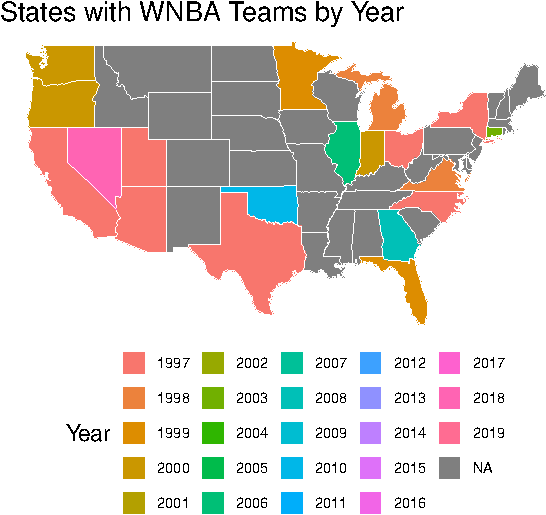
\includegraphics[keepaspectratio]{Health_Proj_files/figure-pdf/unnamed-chunk-2-1.pdf}}

\begin{Shaded}
\begin{Highlighting}[]
\CommentTok{\# Now time series of participation rates in basketball, track, and softball for girls}

\NormalTok{wnba\_states }\OtherTok{\textless{}{-}}\NormalTok{ df\_wnba }\SpecialCharTok{\%\textgreater{}\%}
  \FunctionTok{select}\NormalTok{(team, year) }\SpecialCharTok{\%\textgreater{}\%}
  \FunctionTok{left\_join}\NormalTok{(team\_state, }\AttributeTok{by =} \StringTok{"team"}\NormalTok{) }\SpecialCharTok{\%\textgreater{}\%}
  \FunctionTok{filter}\NormalTok{(}\SpecialCharTok{!}\FunctionTok{is.na}\NormalTok{(state)) }\SpecialCharTok{\%\textgreater{}\%}
  \FunctionTok{mutate}\NormalTok{(}\AttributeTok{state\_num =} \FunctionTok{case\_when}\NormalTok{(}
\NormalTok{    state }\SpecialCharTok{==} \StringTok{"arizona"} \SpecialCharTok{\textasciitilde{}} \DecValTok{3}\NormalTok{,}
\NormalTok{    state }\SpecialCharTok{==} \StringTok{"california"} \SpecialCharTok{\textasciitilde{}} \DecValTok{5}\NormalTok{,}
\NormalTok{    state }\SpecialCharTok{==} \StringTok{"connecticut"} \SpecialCharTok{\textasciitilde{}} \DecValTok{7}\NormalTok{,}
\NormalTok{    state }\SpecialCharTok{==} \StringTok{"florida"} \SpecialCharTok{\textasciitilde{}} \DecValTok{9}\NormalTok{,}
\NormalTok{    state }\SpecialCharTok{==} \StringTok{"georgia"} \SpecialCharTok{\textasciitilde{}} \DecValTok{10}\NormalTok{,}
\NormalTok{    state }\SpecialCharTok{==} \StringTok{"illinois"} \SpecialCharTok{\textasciitilde{}} \DecValTok{13}\NormalTok{,}
\NormalTok{    state }\SpecialCharTok{==} \StringTok{"indiana"} \SpecialCharTok{\textasciitilde{}} \DecValTok{14}\NormalTok{,}
\NormalTok{    state }\SpecialCharTok{==} \StringTok{"michigan"} \SpecialCharTok{\textasciitilde{}} \DecValTok{22}\NormalTok{,}
\NormalTok{    state }\SpecialCharTok{==} \StringTok{"minnesota"} \SpecialCharTok{\textasciitilde{}} \DecValTok{23}\NormalTok{,}
\NormalTok{    state }\SpecialCharTok{==} \StringTok{"nevada"} \SpecialCharTok{\textasciitilde{}} \DecValTok{28}\NormalTok{,}
\NormalTok{    state }\SpecialCharTok{==} \StringTok{"new york"} \SpecialCharTok{\textasciitilde{}} \DecValTok{32}\NormalTok{,}
\NormalTok{    state }\SpecialCharTok{==} \StringTok{"north carolina"} \SpecialCharTok{\textasciitilde{}} \DecValTok{33}\NormalTok{,}
\NormalTok{    state }\SpecialCharTok{==} \StringTok{"ohio"} \SpecialCharTok{\textasciitilde{}} \DecValTok{35}\NormalTok{,}
\NormalTok{    state }\SpecialCharTok{==} \StringTok{"oklahoma"} \SpecialCharTok{\textasciitilde{}} \DecValTok{36}\NormalTok{,}
\NormalTok{    state }\SpecialCharTok{==} \StringTok{"oregon"} \SpecialCharTok{\textasciitilde{}} \DecValTok{37}\NormalTok{,}
\NormalTok{    state }\SpecialCharTok{==} \StringTok{"texas"} \SpecialCharTok{\textasciitilde{}} \DecValTok{43}\NormalTok{,}
\NormalTok{    state }\SpecialCharTok{==} \StringTok{"utah"} \SpecialCharTok{\textasciitilde{}} \DecValTok{44}\NormalTok{,}
\NormalTok{    state }\SpecialCharTok{==} \StringTok{"virginia"} \SpecialCharTok{\textasciitilde{}} \DecValTok{46}\NormalTok{,}
\NormalTok{    state }\SpecialCharTok{==} \StringTok{"washington"} \SpecialCharTok{\textasciitilde{}} \DecValTok{47}
\NormalTok{  )) }\SpecialCharTok{\%\textgreater{}\%}
  \FunctionTok{distinct}\NormalTok{(state\_num, year) }\SpecialCharTok{\%\textgreater{}\%}
  \FunctionTok{filter}\NormalTok{(}\SpecialCharTok{!}\FunctionTok{is.na}\NormalTok{(state\_num))}

\NormalTok{participation\_df }\OtherTok{\textless{}{-}}\NormalTok{ df\_nfhs\_wide }\SpecialCharTok{\%\textgreater{}\%}
  \FunctionTok{filter}\NormalTok{(gender }\SpecialCharTok{==} \DecValTok{1}\NormalTok{) }\SpecialCharTok{\%\textgreater{}\%}
  \FunctionTok{select}\NormalTok{(state, year, Basketball) }\SpecialCharTok{\%\textgreater{}\%}
  \FunctionTok{mutate}\NormalTok{(}\AttributeTok{total =} \FunctionTok{rowSums}\NormalTok{(}\FunctionTok{across}\NormalTok{(}\FunctionTok{where}\NormalTok{(is.numeric)), }\AttributeTok{na.rm =} \ConstantTok{TRUE}\NormalTok{)) }\SpecialCharTok{\%\textgreater{}\%}
  \FunctionTok{mutate}\NormalTok{(}\AttributeTok{basketball\_share =}\NormalTok{ Basketball }\SpecialCharTok{/}\NormalTok{ total) }\SpecialCharTok{\%\textgreater{}\%}
  \FunctionTok{left\_join}\NormalTok{(wnba\_states }\SpecialCharTok{\%\textgreater{}\%} \FunctionTok{mutate}\NormalTok{(}\AttributeTok{has\_wnba =} \DecValTok{1}\NormalTok{), }
            \AttributeTok{by =} \FunctionTok{c}\NormalTok{(}\StringTok{"state"} \OtherTok{=} \StringTok{"state\_num"}\NormalTok{, }\StringTok{"year"}\NormalTok{)) }\SpecialCharTok{\%\textgreater{}\%}
  \FunctionTok{mutate}\NormalTok{(}\AttributeTok{has\_wnba =} \FunctionTok{replace\_na}\NormalTok{(has\_wnba, }\DecValTok{0}\NormalTok{),}
         \AttributeTok{group =} \FunctionTok{ifelse}\NormalTok{(has\_wnba }\SpecialCharTok{==} \DecValTok{1}\NormalTok{, }\StringTok{"WNBA State"}\NormalTok{, }\StringTok{"No WNBA Team"}\NormalTok{)) }\SpecialCharTok{\%\textgreater{}\%}
  \FunctionTok{group\_by}\NormalTok{(group, year) }\SpecialCharTok{\%\textgreater{}\%}
  \FunctionTok{summarise}\NormalTok{(}\AttributeTok{participation\_rate =} \FunctionTok{mean}\NormalTok{(basketball\_share, }\AttributeTok{na.rm =} \ConstantTok{TRUE}\NormalTok{), }\AttributeTok{.groups =} \StringTok{"drop"}\NormalTok{) }\SpecialCharTok{\%\textgreater{}\%}
  \FunctionTok{filter}\NormalTok{(}\SpecialCharTok{!}\FunctionTok{is.na}\NormalTok{(year))}

\FunctionTok{ggplot}\NormalTok{(participation\_df, }\FunctionTok{aes}\NormalTok{(}\AttributeTok{x =}\NormalTok{ year, }\AttributeTok{y =}\NormalTok{ participation\_rate, }\AttributeTok{color =}\NormalTok{ group, }\AttributeTok{group =}\NormalTok{ group)) }\SpecialCharTok{+}
  \FunctionTok{geom\_line}\NormalTok{(}\AttributeTok{linewidth =} \DecValTok{1}\NormalTok{) }\SpecialCharTok{+}
  \FunctionTok{labs}\NormalTok{(}\AttributeTok{title =} \StringTok{"Girls Basketball Participation (Share of Total Participation): WNBA vs Non{-}WNBA States"}\NormalTok{,}
       \AttributeTok{x =} \StringTok{"Year"}\NormalTok{, }\AttributeTok{y =} \StringTok{"Mean Participation"}\NormalTok{, }\AttributeTok{color =} \StringTok{""}\NormalTok{) }\SpecialCharTok{+}
  \FunctionTok{theme\_minimal}\NormalTok{() }\SpecialCharTok{+}
  \FunctionTok{theme}\NormalTok{(}\AttributeTok{legend.position =} \StringTok{"bottom"}\NormalTok{)}
\end{Highlighting}
\end{Shaded}

\pandocbounded{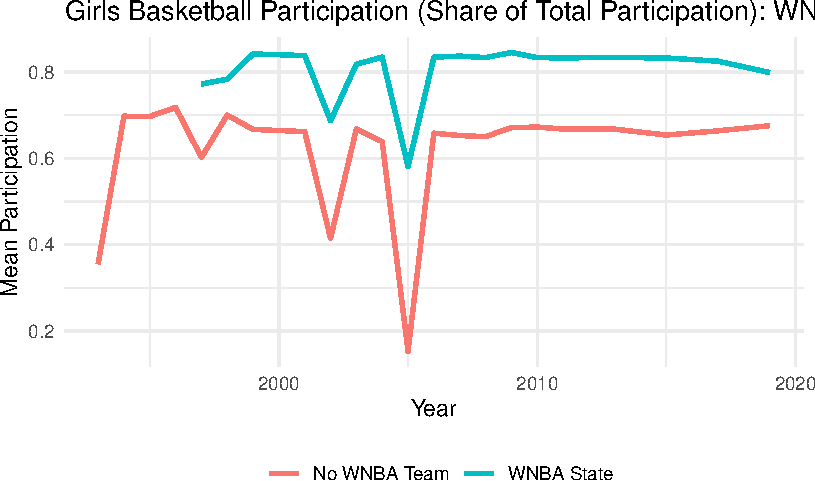
\includegraphics[keepaspectratio]{Health_Proj_files/figure-pdf/unnamed-chunk-3-1.pdf}}

\begin{Shaded}
\begin{Highlighting}[]
\NormalTok{soc\_df }\OtherTok{\textless{}{-}}\NormalTok{ df\_nfhs\_wide }\SpecialCharTok{\%\textgreater{}\%}
  \FunctionTok{filter}\NormalTok{(gender }\SpecialCharTok{==} \DecValTok{1}\NormalTok{) }\SpecialCharTok{\%\textgreater{}\%}
  \FunctionTok{select}\NormalTok{(state, year, Soccer) }\SpecialCharTok{\%\textgreater{}\%}
  \FunctionTok{mutate}\NormalTok{(}\AttributeTok{total =} \FunctionTok{rowSums}\NormalTok{(}\FunctionTok{across}\NormalTok{(}\FunctionTok{where}\NormalTok{(is.numeric)), }\AttributeTok{na.rm =} \ConstantTok{TRUE}\NormalTok{)) }\SpecialCharTok{\%\textgreater{}\%}
  \FunctionTok{mutate}\NormalTok{(}\AttributeTok{soccer\_share =}\NormalTok{ Soccer }\SpecialCharTok{/}\NormalTok{ total) }\SpecialCharTok{\%\textgreater{}\%}
  \FunctionTok{left\_join}\NormalTok{(wnba\_states }\SpecialCharTok{\%\textgreater{}\%} \FunctionTok{mutate}\NormalTok{(}\AttributeTok{has\_wnba =} \DecValTok{1}\NormalTok{), }
            \AttributeTok{by =} \FunctionTok{c}\NormalTok{(}\StringTok{"state"} \OtherTok{=} \StringTok{"state\_num"}\NormalTok{, }\StringTok{"year"}\NormalTok{)) }\SpecialCharTok{\%\textgreater{}\%}
  \FunctionTok{mutate}\NormalTok{(}\AttributeTok{has\_wnba =} \FunctionTok{replace\_na}\NormalTok{(has\_wnba, }\DecValTok{0}\NormalTok{),}
         \AttributeTok{group =} \FunctionTok{ifelse}\NormalTok{(has\_wnba }\SpecialCharTok{==} \DecValTok{1}\NormalTok{, }\StringTok{"WNBA State"}\NormalTok{, }\StringTok{"No WNBA Team"}\NormalTok{)) }\SpecialCharTok{\%\textgreater{}\%}
  \FunctionTok{group\_by}\NormalTok{(group, year) }\SpecialCharTok{\%\textgreater{}\%}
  \FunctionTok{summarise}\NormalTok{(}\AttributeTok{participation\_rate =} \FunctionTok{mean}\NormalTok{(}\StringTok{\textasciigrave{}}\AttributeTok{soccer\_share}\StringTok{\textasciigrave{}}\NormalTok{, }\AttributeTok{na.rm =} \ConstantTok{TRUE}\NormalTok{), }\AttributeTok{.groups =} \StringTok{"drop"}\NormalTok{) }\SpecialCharTok{\%\textgreater{}\%}
  \FunctionTok{filter}\NormalTok{(}\SpecialCharTok{!}\FunctionTok{is.na}\NormalTok{(year)) }
\FunctionTok{ggplot}\NormalTok{(soc\_df, }\FunctionTok{aes}\NormalTok{(}\AttributeTok{x =}\NormalTok{ year, }\AttributeTok{y =}\NormalTok{ participation\_rate, }\AttributeTok{color =}\NormalTok{ group, }\AttributeTok{group =}\NormalTok{ group)) }\SpecialCharTok{+}
  \FunctionTok{geom\_line}\NormalTok{(}\AttributeTok{linewidth =} \DecValTok{1}\NormalTok{) }\SpecialCharTok{+}
  \FunctionTok{labs}\NormalTok{(}\AttributeTok{title =} \StringTok{"Girls Soccer Participation: WNBA vs Non{-}WNBA States"}\NormalTok{,}
       \AttributeTok{x =} \StringTok{"Year"}\NormalTok{, }\AttributeTok{y =} \StringTok{"Mean Participation"}\NormalTok{, }\AttributeTok{color =} \StringTok{""}\NormalTok{) }\SpecialCharTok{+}
  \FunctionTok{theme\_minimal}\NormalTok{() }\SpecialCharTok{+}
  \FunctionTok{theme}\NormalTok{(}\AttributeTok{legend.position =} \StringTok{"bottom"}\NormalTok{)}
\end{Highlighting}
\end{Shaded}

\pandocbounded{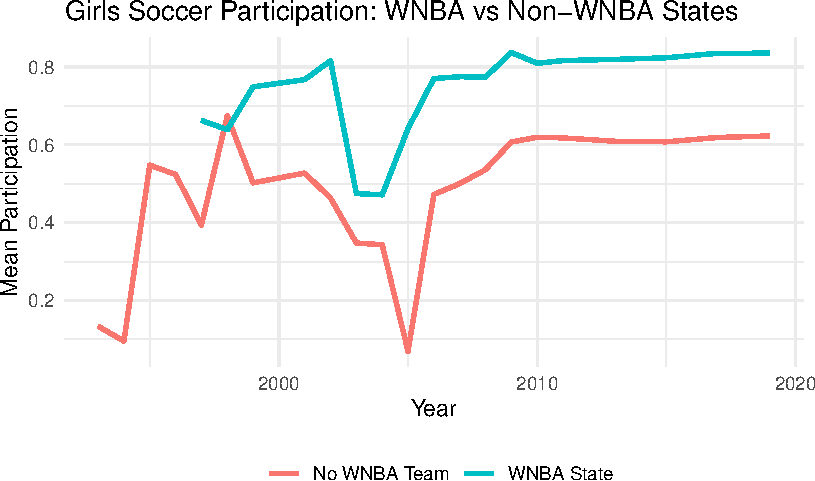
\includegraphics[keepaspectratio]{Health_Proj_files/figure-pdf/unnamed-chunk-3-2.pdf}}

\begin{Shaded}
\begin{Highlighting}[]
\NormalTok{vb\_df }\OtherTok{\textless{}{-}}\NormalTok{ df\_nfhs\_wide }\SpecialCharTok{\%\textgreater{}\%}
  \FunctionTok{filter}\NormalTok{(gender }\SpecialCharTok{==} \DecValTok{1}\NormalTok{) }\SpecialCharTok{\%\textgreater{}\%}
  \FunctionTok{select}\NormalTok{(state, year, Volleyball) }\SpecialCharTok{\%\textgreater{}\%}
  \FunctionTok{mutate}\NormalTok{(}\AttributeTok{total =} \FunctionTok{rowSums}\NormalTok{(}\FunctionTok{across}\NormalTok{(}\FunctionTok{where}\NormalTok{(is.numeric)), }\AttributeTok{na.rm =} \ConstantTok{TRUE}\NormalTok{)) }\SpecialCharTok{\%\textgreater{}\%}
  \FunctionTok{mutate}\NormalTok{(}\AttributeTok{vb\_share =}\NormalTok{ Volleyball }\SpecialCharTok{/}\NormalTok{ total) }\SpecialCharTok{\%\textgreater{}\%}
  \FunctionTok{left\_join}\NormalTok{(wnba\_states }\SpecialCharTok{\%\textgreater{}\%} \FunctionTok{mutate}\NormalTok{(}\AttributeTok{has\_wnba =} \DecValTok{1}\NormalTok{), }
            \AttributeTok{by =} \FunctionTok{c}\NormalTok{(}\StringTok{"state"} \OtherTok{=} \StringTok{"state\_num"}\NormalTok{, }\StringTok{"year"}\NormalTok{)) }\SpecialCharTok{\%\textgreater{}\%}
  \FunctionTok{mutate}\NormalTok{(}\AttributeTok{has\_wnba =} \FunctionTok{replace\_na}\NormalTok{(has\_wnba, }\DecValTok{0}\NormalTok{),}
         \AttributeTok{group =} \FunctionTok{ifelse}\NormalTok{(has\_wnba }\SpecialCharTok{==} \DecValTok{1}\NormalTok{, }\StringTok{"WNBA State"}\NormalTok{, }\StringTok{"No WNBA Team"}\NormalTok{)) }\SpecialCharTok{\%\textgreater{}\%}
  \FunctionTok{group\_by}\NormalTok{(group, year) }\SpecialCharTok{\%\textgreater{}\%}
  \FunctionTok{summarise}\NormalTok{(}\AttributeTok{participation\_rate =} \FunctionTok{mean}\NormalTok{(vb\_share, }\AttributeTok{na.rm =} \ConstantTok{TRUE}\NormalTok{), }\AttributeTok{.groups =} \StringTok{"drop"}\NormalTok{) }\SpecialCharTok{\%\textgreater{}\%}
  \FunctionTok{filter}\NormalTok{(}\SpecialCharTok{!}\FunctionTok{is.na}\NormalTok{(year))}
\FunctionTok{ggplot}\NormalTok{(vb\_df, }\FunctionTok{aes}\NormalTok{(}\AttributeTok{x =}\NormalTok{ year, }\AttributeTok{y =}\NormalTok{ participation\_rate, }\AttributeTok{color =}\NormalTok{ group, }\AttributeTok{group =}\NormalTok{ group)) }\SpecialCharTok{+}
  \FunctionTok{geom\_line}\NormalTok{(}\AttributeTok{linewidth =} \DecValTok{1}\NormalTok{) }\SpecialCharTok{+}
  \FunctionTok{labs}\NormalTok{(}\AttributeTok{title =} \StringTok{"Girls Volleyball Participation: WNBA vs Non{-}WNBA States"}\NormalTok{,}
       \AttributeTok{x =} \StringTok{"Year"}\NormalTok{, }\AttributeTok{y =} \StringTok{"Mean Participation"}\NormalTok{, }\AttributeTok{color =} \StringTok{""}\NormalTok{) }\SpecialCharTok{+}
  \FunctionTok{theme\_minimal}\NormalTok{() }\SpecialCharTok{+}
  \FunctionTok{theme}\NormalTok{(}\AttributeTok{legend.position =} \StringTok{"bottom"}\NormalTok{)}
\end{Highlighting}
\end{Shaded}

\begin{verbatim}
Warning: Removed 3 rows containing missing values or values outside the scale range
(`geom_line()`).
\end{verbatim}

\pandocbounded{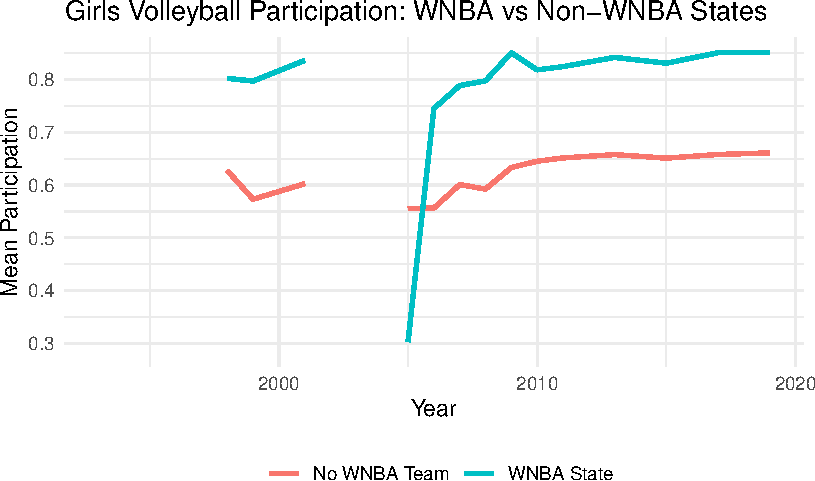
\includegraphics[keepaspectratio]{Health_Proj_files/figure-pdf/unnamed-chunk-3-3.pdf}}

It appears that having a WNBA team in the state leads to a higher
participation rate in sports like basketball, soccer, and volleyball.
There are many confounders here. While population size is one, that is
at least partially controlled for by looking at the share of
participation. Still, there are many other factors that could be at
play, such as the general culture of sports in a given state, the
presence of other sports teams, and the socioeconomic status of the
population. A more rigorous analysis would be needed to establish
causality. To do so, we implement a difference-in-differences
regression, controlling for state and year fixed effects, and clustering
standard errors at the state level. This would allow us to better
isolate the effect of having a WNBA team on girls sports participation,
while controlling for unobserved heterogeneity across states and over
time.

\section{DiD}\label{did}

\(Y_{st} = \beta_0 + \beta_1 \1\{Have WNBA\times Year\} + \delta_s + \gamma_t + \epsilon_{st}\)

\begin{Shaded}
\begin{Highlighting}[]
\FunctionTok{library}\NormalTok{(did)}
\end{Highlighting}
\end{Shaded}

\begin{verbatim}
Warning: package 'did' was built under R version 4.5.2
\end{verbatim}

\begin{verbatim}

Attaching package: 'did'
\end{verbatim}

\begin{verbatim}
The following object is masked from 'package:psych':

    sim
\end{verbatim}

\begin{Shaded}
\begin{Highlighting}[]
\CommentTok{\# Create treatment variable}
\NormalTok{df\_did }\OtherTok{\textless{}{-}}\NormalTok{ df\_nfhs\_wide }\SpecialCharTok{\%\textgreater{}\%}
  \FunctionTok{filter}\NormalTok{(gender }\SpecialCharTok{==} \DecValTok{1}\NormalTok{) }\SpecialCharTok{\%\textgreater{}\%}
  \FunctionTok{left\_join}\NormalTok{(}
\NormalTok{    wnba\_states }\SpecialCharTok{\%\textgreater{}\%} \FunctionTok{group\_by}\NormalTok{(state\_num) }\SpecialCharTok{\%\textgreater{}\%} \FunctionTok{summarise}\NormalTok{(}\AttributeTok{first\_treat =} \FunctionTok{min}\NormalTok{(year)),}
    \AttributeTok{by =} \FunctionTok{c}\NormalTok{(}\StringTok{"state"} \OtherTok{=} \StringTok{"state\_num"}\NormalTok{)}
\NormalTok{  ) }\SpecialCharTok{\%\textgreater{}\%}
  \FunctionTok{mutate}\NormalTok{(}\AttributeTok{first\_treat =} \FunctionTok{replace\_na}\NormalTok{(first\_treat, }\DecValTok{0}\NormalTok{),}
         \AttributeTok{has\_wnba =} \FunctionTok{as.integer}\NormalTok{(first\_treat }\SpecialCharTok{\textgreater{}} \DecValTok{0} \SpecialCharTok{\&}\NormalTok{ year }\SpecialCharTok{\textgreater{}=}\NormalTok{ first\_treat))}

\FunctionTok{library}\NormalTok{(lfe)}
\end{Highlighting}
\end{Shaded}

\begin{verbatim}
Loading required package: Matrix
\end{verbatim}

\begin{verbatim}

Attaching package: 'Matrix'
\end{verbatim}

\begin{verbatim}
The following objects are masked from 'package:tidyr':

    expand, pack, unpack
\end{verbatim}

\begin{Shaded}
\begin{Highlighting}[]
\NormalTok{did\_model }\OtherTok{\textless{}{-}} \FunctionTok{felm}\NormalTok{(Basketball }\SpecialCharTok{\textasciitilde{}}\NormalTok{ has\_wnba }\SpecialCharTok{|}\NormalTok{ state }\SpecialCharTok{+}\NormalTok{ year }\SpecialCharTok{|} \DecValTok{0} \SpecialCharTok{|}\NormalTok{ state,}
                  \AttributeTok{data =}\NormalTok{ df\_did)}
\FunctionTok{summary}\NormalTok{(did\_model)}
\end{Highlighting}
\end{Shaded}

\begin{verbatim}

Call:
   felm(formula = Basketball ~ has_wnba | state + year | 0 | state,      data = df_did) 

Residuals:
   Min     1Q Median     3Q    Max 
-56410   -600    -96    501  56251 

Coefficients:
         Estimate Cluster s.e. t value Pr(>|t|)
has_wnba     1128         1154   0.978    0.333

Residual standard error: 4788 on 763 degrees of freedom
  (379 observations deleted due to missingness)
Multiple R-squared(full model): 0.7337   Adjusted R-squared: 0.7089 
Multiple R-squared(proj model): 0.002546   Adjusted R-squared: -0.09027 
F-statistic(full model, *iid*):29.61 on 71 and 763 DF, p-value: < 2.2e-16 
F-statistic(proj model): 0.9557 on 1 and 49 DF, p-value: 0.3331 
\end{verbatim}




\end{document}
